\documentclass[10pt]{article}
\usepackage[a4paper,margin=2.2cm]{geometry}
\usepackage[T1]{fontenc}
\usepackage{lmodern}
\usepackage{microtype}
\usepackage{amsmath,amssymb,mathtools}
\usepackage{booktabs}
\usepackage{graphicx}
\usepackage{xcolor}
\usepackage{colortbl}
\usepackage[font=small,labelfont=bf]{caption}
\usepackage{subcaption}
\usepackage[section,above]{placeins}   % floats never cross a section boundary
\usepackage{enumitem}
\usepackage{algorithm}
\usepackage{algorithmic}
\usepackage{tikz}
\usetikzlibrary{arrows.meta,positioning,fit,calc}
\usepackage[numbers,sort&compress]{natbib}
\usepackage[colorlinks=true,linkcolor=blue!50!black,citecolor=blue!50!black,urlcolor=blue!50!black]{hyperref}

\definecolor{ours}{HTML}{2A78D6}
\definecolor{muonc}{HTML}{EB6834}
\newcommand{\method}{StreamMuon}\newcommand{\lite}{StreamMuon-Lite}
\newcommand{\R}{\mathbb{R}}
\setlist{nosep,leftmargin=1.4em}

\title{Eliminating the Gradient Buffer:\\ Algebraically Exact In-Backward Momentum\\ with Two-Thirds Less Memory for Dense and Routed Models}
\author{Ammar Patel\\ Independent Researcher}
\date{\today}

\begin{document}
\maketitle

\begin{abstract}
Training with gradient accumulation keeps a full-size gradient buffer next to the weights and optimizer state: 16 bytes
per parameter with AdamW and 12 with Muon, before any activation is stored. We show that for momentum optimizers this
buffer is unnecessary. Each micro-batch's gradient is folded into the momentum during the backward pass and freed, with
micro-batch weights that make the result equal to accumulate-then-update, and a snapshot of the previous
momentum (about one byte per parameter) recovers Nesterov momentum, the global gradient norm and clipping, all exact in exact arithmetic. The same byte can
instead hold an int8 running mean of the update's gradient, a quarter of a full-precision buffer, which keeps the norm
exact even under abrupt gradient changes; we recommend it in practice. With momentum
in blockwise int8 and weights in bf16, both stochastically rounded, a weight matrix's training state falls by 67\%
against Muon and 75\% against AdamW (12 and 16 to 4 bytes per parameter; without the snapshot 3 bytes, $-$75\% and
$-$81\%); the update rule is unchanged up to the precision of its gradients (bf16), its state (int8) and the Newton--Schulz iterations (fp8). For mixture-of-experts layers the absorb runs
inside the grouped weight-gradient kernel and each expert's momentum is clocked by the tokens it receives. With Muon's
update (StreamMuon), a 113M Transformer comes within 0.008 bits per byte of Muon's loss (1.147 vs 1.139), and with the one-byte accumulator, over three seeds, within 0.003 (1.148$\pm$0.007 vs 1.145$\pm$0.007), less than half the seed-to-seed spread;
streaming costs no throughput (StreamMuon runs at the speed of Muon with the same Newton--Schulz kernels), and where Muon
must recompute activations to fit, StreamMuon is 1.18--1.22$\times$ faster. On a standard mixture-of-experts
Transformer it also matches Muon (1.131 with the one-byte accumulator and 1.135 with the snapshot, vs 1.126), and with SGD-Nesterov on CIFAR-10 the streamed form
matches fp32 SGD (85.9 vs 86.4\%, three seeds). On
one 8\,GB GPU, AdamW, Muon and 8-bit Muon stop at 0.28B dense parameters, whose training state at 2B would be 32, 24 and
18\,GB; StreamMuon runs 25 training updates at 1.46B parameters (5.2$\times$) and its lighter variant at 2.0B (7.1$\times$,
6\,GB of state), with activation checkpointing; for a standard mixture-of-experts Transformer the largest
model grows from 0.51B (8-bit Muon) to 1.31B (StreamMuon) and 1.71B (Lite).
\end{abstract}





\section{Introduction}
The minimum hardware a training run needs is set by its static memory: weights, gradients and optimizer state, paid for
every parameter at every step. Compute decides how long a run takes; static memory decides how many accelerators it
must be spread over before it can start, and what is left for activations, batch and context. With
AdamW~\citep{loshchilov2019adamw} in mixed precision this is 16 bytes per parameter; with
Muon~\citep{jordan2024muon,liu2025muonscalable}, which keeps one moment instead of two, about 12. Mixture-of-experts
(MoE) models~\citep{shazeer2017moe} sharpen the problem: compute follows the active parameters, static memory the
total.

Optimizer research has mostly competed on quality per token, and those gaps shrink with scale: against a carefully
tuned AdamW, Muon-type speedups fall from about 1.3--1.4$\times$ at 0.1B parameters to about 1.1$\times$ at
1.2B~\citep{wen2026fantastic}. Static memory does not shrink; it stays at 12--16 bytes per parameter at any scale.

\begin{figure}[!t]
\centering
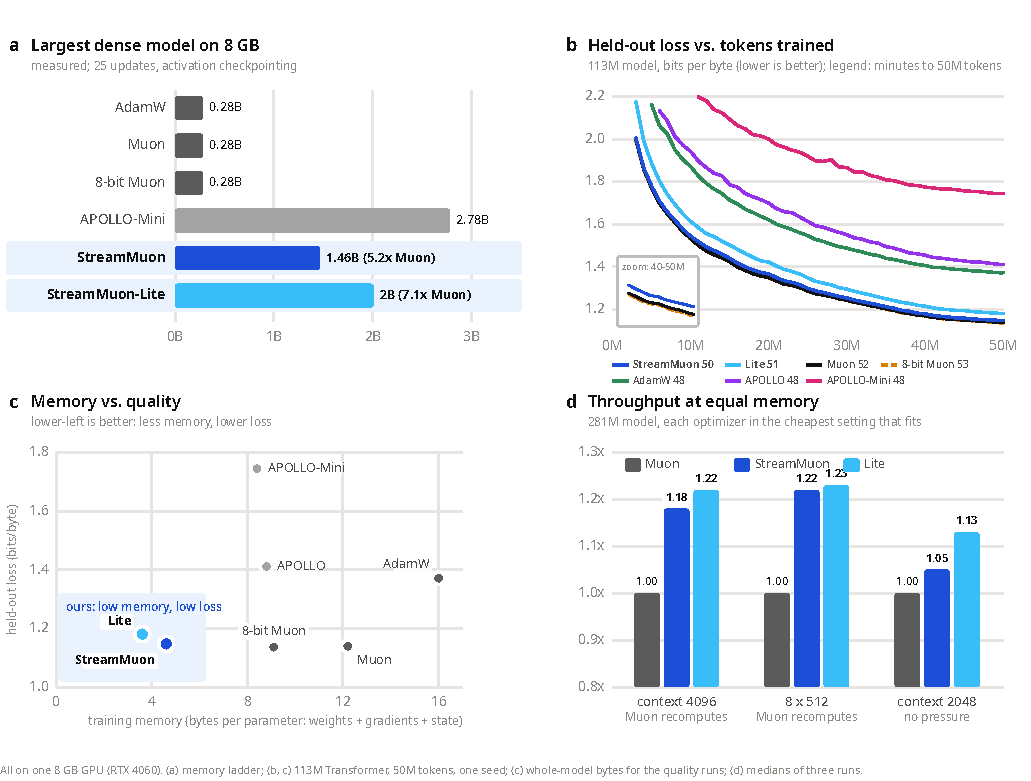
\includegraphics[width=\linewidth]{fig/fig1_v2.pdf}
\caption{\method{} against AdamW, Muon, 8-bit Muon and APOLLO on one 8\,GB GPU. (a) Largest dense Transformer each
optimizer trains (25 updates, activation checkpointing for every optimizer); APOLLO-Mini's larger capacity comes with
the highest loss (c). (b) Held-out loss of a 113M model against
tokens trained (same data and schedule for all), one colour per optimizer, with each run's wall-clock time to 50M
tokens in the legend, including APOLLO at rank $d/4$ (1.411 at the end) and APOLLO-Mini (1.745); the inset zooms on the last
10M tokens, where Muon, 8-bit Muon and \method{}
lie within about 0.01 bits per byte of each other (1.136--1.147). (c) Training memory (whole-model bytes per parameter of
weights, gradients and optimizer state of the 113M quality runs; Table~\ref{tab:glance} gives the weight-matrix limit)
against final held-out loss, including APOLLO at rank $d/4$: only \method{} combines Muon-level loss with
less than half of Muon's memory. (d) Throughput of a
281M model when each optimizer uses the cheapest setting that fits the GPU (Muon $=1$; medians of three runs): in
the first two settings Muon needs activation checkpointing to fit and \method{} and \lite{} do not; in the third none
of them checkpoints (Table~\ref{tab:iso}).}
\label{fig:memscale}\label{fig:capacity}\label{fig:ladder}\label{fig:lm}
\end{figure}

\begin{table}[!tb]
\centering\small
\caption{At a glance: 113M Transformer, 50M tokens (loss, speed) and one 8\,GB GPU (capacity). Differences are
relative to Muon. Bytes: training state of a weight matrix (weights, gradients, optimizer state), the large-model limit.
APOLLO-Mini's 2.0 is its layer-wise bf16 form, used for capacity; its quality run keeps fp32 weights and a gradient
buffer (8.4 bytes per parameter for the whole model, Table~\ref{tab:lm}).}
\label{tab:glance}
\setlength{\tabcolsep}{4.5pt}
\begin{tabular}{lcccccc}
\toprule
& \multicolumn{2}{c}{held-out bits/byte} & speed & \multicolumn{2}{c}{bytes per parameter} & largest dense \\
optimizer & value & vs Muon & vs Muon & value & vs Muon & model on 8\,GB \\
\midrule
AdamW & 1.371 & +0.232 & 1.07$\times$ & 16.0 & +33\% & 0.28B \\
Muon & 1.139 & -- & 1.00$\times$ & 12.0 & -- & 0.28B \\
8-bit Muon & 1.136 & $-$0.003 & 0.99$\times$ & 9.0 & $-$25\% & 0.28B \\
APOLLO-Mini & 1.745 & +0.606 & 1.09$\times$ & 2.0 & $-$83\% & 2.78B \\
\rowcolor{ours!12} \textbf{\method{}} & \textbf{1.147} & \textbf{+0.008} & \textbf{1.04$\times$} & \textbf{4.0} & \textbf{$-$67\%} & \textbf{1.46B (5.2$\times$)} \\
\rowcolor{ours!12} \quad one-byte accumulator$^\S$ & 1.142 & +0.003 & 1.03$\times$ & 4.0 & $-$67\% & -- \\
\rowcolor{ours!12} \textbf{\lite{}} & 1.180 & +0.041 & 1.02$\times$ & \textbf{3.0} & \textbf{$-$75\%} & \textbf{2.0B (7.1$\times$)} \\
\bottomrule
\end{tabular}\\[2pt]
{\footnotesize $^\S$The recommended form (\S\ref{sec:exact}); its capacity was not measured separately; it keeps the same bytes per
parameter as \method{}, and at 113M its measured peak memory is the same (4.17\,GB, Table~\ref{tab:lm}). APOLLO at rank $d/4$: 1.411 bits per byte. Seed 0. Over three seeds Muon reaches 1.145$\pm$0.007 and the one-byte accumulator 1.148$\pm$0.007; paired by seed, the accumulator trails Muon by 0.003$\pm$0.0005. Speed: cumulative tokens per second, including StreamMuon's fp8 Newton--Schulz (\S\ref{sec:lm}). Routed: on a standard MoE Transformer (148.6M total) Muon reaches 1.126,
\method{} 1.131 (one-byte accumulator) / 1.135 (snapshot); in the width-1024 MoE ladder Muon fits no rung (it trains only the 0.15B quality
model), 8-bit Muon 0.51B, \method{} 1.31B and \lite{} 1.71B.}
\end{table}

The largest of the three pieces that is not needed is the gradient buffer. Under gradient accumulation, a standard
implementation sums each micro-batch's gradient into a full-precision buffer and hands the sum to the optimizer. For
momentum optimizers the sum is only ever used inside an exponential average, so it can be folded into the momentum as
it is produced, during the backward pass, and freed. Doing this exactly, with low-precision state, and for routed
experts is the subject of this paper. Our contributions:
\begin{enumerate}
  \item \textbf{Streaming accumulation without a gradient buffer}: micro-batch gradients absorbed into blockwise int8
  momentum during backward with token-count weights that equal accumulate-then-update exactly, for any number of
  micro-batches; for MoE layers inside the grouped weight-gradient kernel, so expert gradients are never written to
  memory (\S\ref{sec:stream}).
  \item \textbf{Algebraically exact Nesterov momentum, gradient norm and clipping} from a one-byte snapshot of the
  previous momentum (\S\ref{sec:exact}), for dense matrices and routed experts.
  \item \textbf{Token-clock momentum for routed experts}: each expert's momentum horizon and step counted in the tokens
  it receives (\S\ref{sec:clock}); a mechanism that cuts rare-expert drift tenfold, not yet shown to improve quality.
  \item \textbf{Measurements in a memory-bound regime}: quality and throughput against Muon, AdamW, 8-bit Muon and
  APOLLO, with the Newton--Schulz path controlled; the largest dense and routed models each optimizer can train; and
  throughput at equal memory (\S\ref{sec:results}).
\end{enumerate}
Two of the pieces are known and we build on them: blockwise int8 optimizer states~\citep{dettmers2022eightbit,gupta2025muon8}
and bf16 weights with stochastic rounding~\citep{zamirai2020bf16,ozkara2025sr}. Together with streaming, the training
state of a weight matrix falls from 12 to 4.0 bytes per parameter (Figure~\ref{fig:bytes}): weights 4$\to$2 (bf16),
gradient buffer 4$\to$0 (streaming, ours), momentum 4$\to$1 (int8) plus the 1-byte snapshot that makes the streamed
update exact (ours). The techniques act on the optimizer's \emph{state}; the update rule is unchanged up to the
precision of that state. We measure them with Muon's update rule (StreamMuon) and, on CIFAR-10, with SGD-Nesterov.

% ======================================================================================================
\section{Where training memory goes}
\label{sec:background}
Table~\ref{tab:bytes} defines the bytes per parameter used throughout: what each optimizer holds between the backward
pass and the update, for the whole 113M model (where fp32 embeddings and norms and the output head's AdamW state add a
little) and for weight matrices alone (the large-model limit).

\begin{table}[!t]
\centering\small
\caption{Bytes per parameter held during training (activations excluded), measured from the optimizer state of the
113M Transformer quality runs. The matrix column is the large-model limit used in Table~\ref{tab:glance} and
Section~\ref{sec:scale}.}
\label{tab:bytes}
\setlength{\tabcolsep}{4pt}
\begin{tabular}{lccccc}
\toprule
optimizer & weights & gradients & state & whole model & matrices \\
\midrule
AdamW (fp32 weights, $m$, $v$) & 4.0 & 4.0 & 8.0 & 16.0 & 16.0 \\
Muon (fp32 weights, momentum) & 4.0 & 4.0 & 4.18 & 12.2 & 12.0 \\
8-bit Muon~\citep{gupta2025muon8} (fp32, int8 momentum) & 4.0 & 4.0 & 1.32 & 9.3 & 9.0 \\
APOLLO-Mini~\citep{zhu2025apollo} (rank 1, layer-wise) & 2.0 & -- & $\approx$0 & -- & 2.0 \\
\lite{} (bf16, int8 momentum, streaming) & 2.09 & 0.18$^\dagger$ & 1.33 & \textbf{3.6} & \textbf{3.0} \\
\method{} (+ int8 snapshot$^\ddagger$) & 2.09 & 0.18$^\dagger$ & 1.33 + 0.96 & 4.6 & 4.0 \\
\bottomrule
\end{tabular}\\[2pt]
{\footnotesize $^\dagger$Embeddings, norms and the output head keep fp32 gradients; a weight matrix's bf16 gradient exists
only between its backward and its absorb, one matrix at a time (an expert's is never written). $^\ddagger$Taken at an
update's first micro-batch and released at the update, so present during the backward passes; the measured
whole-model value is below 1.016 because non-matrix parameters have no snapshot.}
\end{table}

\begin{table}[!t]
\centering\small
\caption{Which piece saves what, per weight matrix, with the largest dense model each configuration trains on the
8\,GB GPU (25 updates, activation checkpointing). The matched low-precision row has our weights and momentum but keeps
the accumulated gradient buffer. Streaming removes the accumulated buffer, not each matrix's transient gradient.}
\label{tab:matched}
\setlength{\tabcolsep}{4pt}
\begin{tabular}{lccccc}
\toprule
configuration & weights & gradient buffer & momentum & snapshot & bytes / largest \\
\midrule
Muon & fp32 & fp32 & fp32 & -- & 12 / 0.28B \\
8-bit Muon & fp32 & fp32 & int8 & -- & 9 / 0.28B \\
matched low precision & bf16 & bf16 & int8 & -- & 5 / 0.61B \\
\rowcolor{ours!12} \method{} & bf16 & none (streamed) & int8 & int8 & 4 / 1.46B \\
\rowcolor{ours!12} \lite{} & bf16 & none (streamed) & int8 & -- & 3 / 2.0B \\
\bottomrule
\end{tabular}
\end{table}

\begin{figure}[!t]
\centering
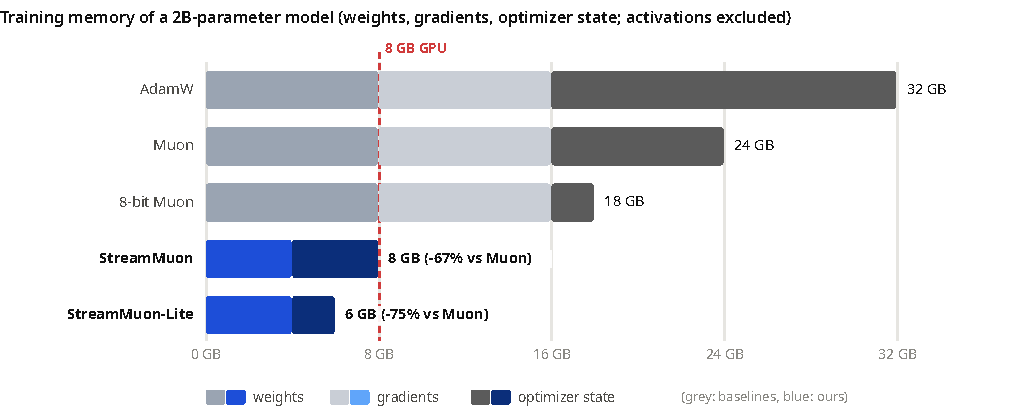
\includegraphics[width=\linewidth]{fig/f2_bytes.pdf}
\caption{Where the memory goes, per component, for a 2B-parameter model (weight matrices; activations excluded). Per
weight matrix \method{} needs 67\% less than Muon and \lite{} 75\% less: weights halve (bf16, prior work), the accumulated gradient
buffer disappears (streaming; a matrix's own gradient still exists briefly, one matrix at a time) and the state shrinks to one or two int8 bytes (int8 momentum, prior work, plus our snapshot). \lite{} trains this model on the 8\,GB GPU (7.26\,GB
peak including activations).}
\label{fig:bytes}
\end{figure}

% ======================================================================================================
\section{Method}
\label{sec:method}

\subsection{Overview}
\label{sec:rule}
\method{} keeps Muon's update rule. For each weight matrix $W\in\R^{m\times n}$ (or expert slice) the direction is the
orthogonal polar factor of the momentum (or of its Nesterov form), computed by five quintic Newton--Schulz iterations,
\begin{equation}
  X_0 = Y/\|Y\|_F,\qquad X_{j+1}=aX_j+b\,(X_jX_j^{\top})X_j+c\,(X_jX_j^{\top})^2X_j,\qquad (a,b,c)=(3.4445,-4.7750,2.0315),
  \label{eq:ns}
\end{equation}
and the weights take the step
\begin{equation}
  W \leftarrow \mathrm{SR}_{\mathrm{bf16}}\!\big(W-\eta\,\psi\,(0.2\sqrt{\max(m,n)}\,X_5+\lambda W)\big),
  \label{eq:wd}
\end{equation}
with $\psi=1$ for dense matrices and the token-clock factor for experts (\S\ref{sec:clock}); embeddings, the output head
and vectors use AdamW ($\beta_2=0.95$). Table~\ref{tab:pieces} lists which pieces depend on the update rule. The two
variants differ only in the snapshot: \method{} keeps an int8 snapshot of the previous momentum during the update for
exact Nesterov momentum, gradient norm and clipping; \lite{} keeps none, which drops Nesterov momentum and estimates
the clipping norm one update late.

\begin{table}[!t]
\centering\small
\caption{Which pieces depend on the update rule. The algebra holds for any first-moment state; quality with int8 state
was measured with Muon's update and, on CIFAR-10, with SGD-Nesterov (Appendix~\ref{app:tasks}); it depends on how
sensitive a rule is to rounding noise (\S\ref{sec:limits}).}
\label{tab:pieces}
\begin{tabular}{p{0.52\linewidth}p{0.4\linewidth}}
\toprule
piece & applies to \\
\midrule
blockwise int8 momentum; bf16 weights with stochastic rounding; streaming absorb with equal micro-batch weights;
snapshot for exact Nesterov, norm and clipping; token-clock momentum & any optimizer whose state is an EMA of gradients \\
fp8 Newton--Schulz & Muon-type (polar) updates \\
streaming of a second moment & not exact: per-micro-batch squares differ from the square of the mean, so an Adam
version would change its estimator \\
\bottomrule
\end{tabular}
\end{table}

\subsection{Int8 momentum and bf16 weights}
\label{sec:int8}
\label{sec:sr}
$M$ is stored as int8 values $q$ with one bf16 scale per block of 128 entries,
$s_B=\mathrm{bf16}\big(\max_{i\in B}|m_i|\,(1+2^{-7})/127\big)$, $q_i=\mathrm{SR}(m_i/s_B)\in[-127,127]$: 1.016 bytes per
parameter. The factor $1+2^{-7}$ keeps the rounded scale above the block maximum, so no entry is clipped; stochastic
rounding (SR) keeps the momentum unbiased even when an update is below one quantization step, which avoids the
stalling of low-precision EMA states~\citep{topollai2026staleness}. Matrices are stored only in bf16, and the fp32 result
of \eqref{eq:wd} is rounded stochastically, so small updates survive in expectation~\citep{zamirai2020bf16,ozkara2025sr}.

\subsection{Streaming: gradients into momentum during backward}
\label{sec:stream}
With $K$ micro-batches per update, a standard implementation sums $K$ gradients into a buffer. \method{} instead updates
$M$ after each micro-batch and frees the gradient. With a running token count,
\begin{equation}
  M_k=\frac{(\tau+n_{<k})\,M_{k-1}+S_k}{\tau+n_{\le k}},\qquad\text{i.e.}\quad M_k=b_kM_{k-1}+(1-b_k)\,\hat g_k,\quad
  b_k=\frac{\tau+n_{<k}}{\tau+n_{\le k}},
  \label{eq:equal}
\end{equation}
where $S_k$ is micro-batch $k$'s summed per-token gradient, $\hat g_k$ its mean, $n_{<k}$ and $n_{\le k}$ the tokens
before and including it, and $\tau=\tfrac{\beta}{1-\beta}N$ for an update of $N$ tokens. The factors telescope, so after
the update $M_t=\beta M_{t-1}+(1-\beta)\bar G_t$ in exact arithmetic, with no extra state (Appendix~\ref{app:deriv};
Figure~\ref{fig:stream}); with int8 state each absorb adds unbiased rounding. For dense matrices our implementation
counts micro-batches instead of tokens ($n$ in micro-batches), which equals the token form for the equal-length
packed micro-batches of all our pre-training runs and matches the usual average of micro-batch losses otherwise;
experts use token counts (\S\ref{sec:clock}). Dequantization, the update, requantization and the squared norm run in one Triton kernel
per matrix and micro-batch. The coefficients $b_k$, the Nesterov factor $a=\prod_k b_k$ and the first-visit flag are
computed on the host, and the kernel treats each matrix as rows of 128 entries (the int8 scale blocks), so any shape
takes the same path; this one launch replaced about 35 small ones and cut the absorb from 39 to 3.3\,ms per micro-batch
at 113M parameters. \lite{} estimates the global gradient norm from per-micro-batch norms, $(\sum_k\|\hat g_k\|^2)^{1/2}/K$ (an
underestimate by up to $\sqrt K$ when micro-batch gradients agree, an overestimate, without bound, when they cancel), and applies the
clipping coefficient one update late, to the next update's micro-batches.

\paragraph{MoE: absorb in the GEMM epilogue.} Routed experts are computed with grouped GEMMs. In the backward pass each
expert's weight-gradient tile is produced in registers by the grouped $\mathrm{d}W$ kernel; we absorb it into that
expert's int8 momentum in the kernel's epilogue, so the expert gradient is never written to memory.

\begin{figure}[!t]
\centering
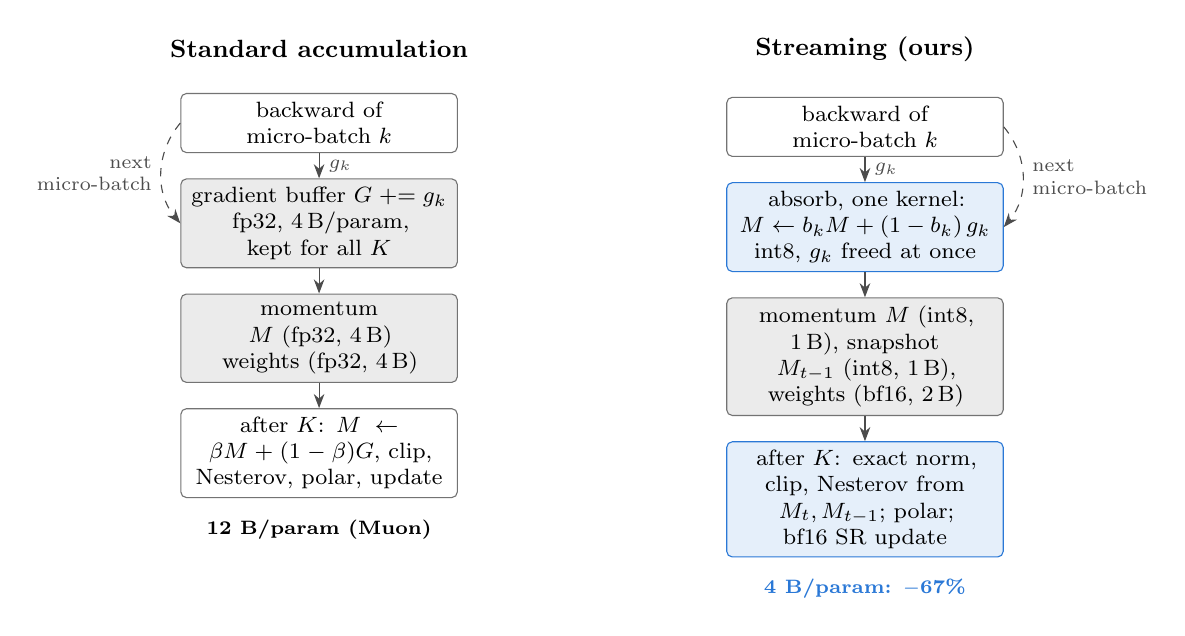
\begin{tikzpicture}[font=\footnotesize, node distance=3.2mm,
  box/.style={draw=black!55, rounded corners=2pt, align=center, inner sep=3pt, minimum height=7.5mm, fill=white, text width=33mm},
  mem/.style={draw=black!55, rounded corners=2pt, align=center, inner sep=3pt, minimum height=7.5mm, fill=black!8, text width=33mm},
  hl/.style={draw=ours, rounded corners=2pt, align=center, inner sep=3pt, minimum height=7.5mm, fill=ours!12, text width=33mm},
  arr/.style={-{Stealth[length=1.8mm]}, black!70}]
% standard
\node[font=\small\bfseries] (tA) {Standard accumulation};
\node[box, below=of tA] (bA) {backward of micro-batch $k$};
\node[mem, below=of bA] (gA) {gradient buffer $G \mathrel{+}= g_k$\\fp32, 4\,B/param, kept for all $K$};
\node[mem, below=of gA] (mA) {momentum $M$ (fp32, 4\,B)\\weights (fp32, 4\,B)};
\node[box, below=of mA] (uA) {after $K$: $M\leftarrow\beta M+(1-\beta)G$, clip, Nesterov, polar, update};
\draw[arr] (bA) -- node[right, font=\scriptsize]{$g_k$} (gA);
\draw[arr] (gA) -- (mA); \draw[arr] (mA) -- (uA);
\draw[arr, dashed] (bA.west) to[bend right=40] node[left, font=\scriptsize, align=right]{next\\micro-batch} (gA.west);
% streaming
\node[font=\small\bfseries, right=34mm of tA] (tB) {Streaming (ours)};
\node[box, below=of tB] (bB) {backward of micro-batch $k$};
\node[hl, below=of bB] (aB) {absorb, one kernel: $M \leftarrow b_k M + (1-b_k)\,g_k$\\int8, $g_k$ freed at once};
\node[mem, below=of aB] (mB) {momentum $M$ (int8, 1\,B), snapshot $M_{t-1}$ (int8, 1\,B), weights (bf16, 2\,B)};
\node[hl, below=of mB] (uB) {after $K$: exact norm, clip, Nesterov from $M_t, M_{t-1}$; polar; bf16 SR update};
\draw[arr] (bB) -- node[right, font=\scriptsize]{$g_k$} (aB);
\draw[arr] (aB) -- (mB); \draw[arr] (mB) -- (uB);
\draw[arr, dashed] (bB.east) to[bend left=40] node[right, font=\scriptsize, align=left]{next\\micro-batch} (aB.east);
\node[below=1.5mm of uA, font=\scriptsize\bfseries] {12 B/param (Muon)};
\node[below=1.5mm of uB, font=\scriptsize\bfseries, text=ours] {4 B/param: $-$67\%};
\end{tikzpicture}
\caption{Gradient accumulation with and without a gradient buffer, per weight matrix. Left: the standard form keeps a
full-precision gradient buffer for all $K$ micro-batches. Right: each micro-batch's gradient is folded into the int8 momentum as
soon as it is produced and freed; at the update, the momentum and a one-byte snapshot of its previous value give the
exact norm, clip and Nesterov direction. For MoE experts the absorb runs inside the grouped weight-gradient kernel, so the
expert gradient is never written to memory.}
\label{fig:stream}
\end{figure}


\subsection{Exact Nesterov momentum, norm and clipping}
\label{sec:exact}
\method{} snapshots $M_{t-1}$ (int8, 1.016\,B/param) at the first absorb of each update and absorbs gradients
unclipped. With $M_t=aM_{t-1}+(1-a)\bar G_t$ ($a=\beta$ for dense matrices, the token-clock decay for experts), the exact
gradient norm is $\|\bar G_t\|=\|M_t-aM_{t-1}\|/(1-a)$; the clipping coefficient $\kappa_t\le1$ is applied once,
\begin{equation}
  M_t \leftarrow aM_{t-1}+\kappa_t\,(M_t-aM_{t-1}),
  \label{eq:exactclip}
\end{equation}
which is exactly the momentum that clipping the update's gradient would have produced, without amplifying rounding
noise; and the Nesterov direction is
\begin{equation}
  D_t \;=\; aM_t+(1-a)\kappa_t\bar G_t \;=\; (1+a)\,M_t-a\,M_{t-1}.
  \label{eq:nesterov}
\end{equation}
Independent rounding of $M_t$ and $M_{t-1}$ gives $D_t$ about $4.7\times$ the rounding variance of one int8 momentum,
still far below the gradient noise. All three run in one fused pass.

\paragraph{Algebra and implementation.} Two results should be kept apart. Algebraically, Eqs.~\ref{eq:equal}--\ref{eq:nesterov}
are exact: with exact gradients and state, streaming reproduces accumulate-then-update, its norm, its clip and its
Nesterov direction. Numerically, our implementation adds three approximations: matrix gradients are bf16, the
momentum and snapshot are int8 (stochastically rounded, unbiased), and the first Newton--Schulz iterations run in
fp8. In the norm, the division by $1-a$ amplifies the int8 rounding of $M_t$ and $M_{t-1}$ ($20\times$ at
$\beta=0.95$, more as $\beta\to1$). Without int8 rounding, against a non-streaming reference with gradient scales varying
$50\times$, the update matches within 3\% and the norm within 2\%. With int8 momentum the norm's error depends on how
fast the gradient scale changes: in our 113M runs the logged gradient norms of \method{} are about 5\% above Muon's
(median ratio over the last five-sixths of training; 4\% for the one-byte accumulator below); in a stress test where the gradient scale drops $50\times$ within three updates, the
rounding of the old momentum dominates and the norm is overestimated up to $9\times$, so those updates are clipped too
strongly (Muon's update direction is invariant to scale; only the mix of new gradient and old momentum changes). The
one-byte accumulator variant below reads the norm directly and is exact to 0.1\% in the same stress test; it is the
better choice where gradient scales change abruptly.

\paragraph{What the global norm covers.} The clipping norm is global over the whole model: dense weight matrices
contribute exactly through the snapshot identity above; the parameters trained by AdamW (embeddings, norms, the output
head) contribute their gradients, which are present at the update and are clipped by the same coefficient in the same
update. Routed experts, whose gradients are never stored, contribute exactly as well: per expert, the snapshot (or
the one-byte accumulator) gives the update's token-weighted mean gradient in token-clock units (\S\ref{sec:clock}), and
the weight $n_s/N$ maps it back to the gradient of the mean loss. Since $1-a_s=n_s/(\tau+n_s)$ after an expert's first
update, its term is $((\tau+n_s)/N)^2\|M_{s,t}-a_sM_{s,t-1}\|^2$: the int8 rounding is amplified by about
$\tfrac{\beta}{1-\beta}f_{\mathrm{ref}}$ (about 5 for top-2 of 8 experts) instead of $1/(1-\beta)=20$ for a dense matrix. Against a plainly accumulated reference with uneven
and idle experts, the streamed global norm agrees within 2\% with the one-byte accumulator and within 6\% with the
int8 snapshot; the in-kernel absorb and the hook path agree within rounding noise.

\begin{figure}[!t]
\centering\small
\fbox{\begin{minipage}{0.95\linewidth}
\textbf{One update of \method{} with $K$ micro-batches} (dense matrices; experts as noted in the text)
\begin{enumerate}\itemsep0pt
\item At the first absorb of the update, copy the int8 momentum $M_{t-1}$ to the snapshot (per matrix, as its first gradient arrives).
\item For $k=1..K$: backward of micro-batch $k$; as each matrix's bf16 gradient is complete, one kernel folds it into
$M$ with weight $1-b_k$ (Eq.~\ref{eq:equal}), unclipped, requantizes $M$ to int8 and frees the gradient.
\item After the last backward, one global reduction: $\|\bar G_t\|^2=\sum_{\text{dense}}\|M_t-aM_{t-1}\|^2/(1-a)^2$
$+\,\|g\|^2$ of the AdamW-managed parameters (+ each expert's snapshot term, weighted by $(n_s/N)^2$). One coefficient $\kappa_t=\min(1,c/\|\bar G_t\|)$.
\item AdamW parameters: gradients scaled by $\kappa_t$, AdamW step.
\item Per matrix, one fused pass: clip (Eq.~\ref{eq:exactclip}), Nesterov direction (Eq.~\ref{eq:nesterov}), int8
requantization of $M_t$; then batched Newton--Schulz (Eq.~\ref{eq:ns}) and the bf16 stochastically rounded step
(Eq.~\ref{eq:wd}); the snapshot is released.
\end{enumerate}
\end{minipage}}
\caption{Order of operations. The only global synchronization is the norm reduction in step 3, which reads the int8
momentum and snapshot. No accumulated gradient buffer exists for the weight matrices; each matrix's gradient lives
only until its absorb.}
\label{fig:algo}
\end{figure}

\paragraph{Variant: a one-byte gradient accumulator.} The same byte can hold the update's mean gradient $\bar G_t$
instead of $M_{t-1}$: each micro-batch is absorbed into a fresh int8 running mean (weights $(k-1)/k$), and at the update
$M_t=aM_{t-1}+(1-a)\kappa_t\bar G_t$, $\|\bar G_t\|$ is read directly and the Nesterov direction is
$D_t=aM_t+(1-a)\kappa_t\bar G_t=a^2M_{t-1}+(1-a^2)\kappa_t\bar G_t$. This form keeps a gradient buffer, one byte
instead of four, and reads the norm without the $1/(1-a)$ amplification; its rounding variance in $D_t$ is about
$4\times$ lower than the snapshot form's ($a^4\sigma_M^2+(1-a^2)^2\kappa_t^2\sigma_G^2$ against $((1+a)^2+a^2)\sigma_M^2$, for
noise-dominated gradients). It is implemented for dense matrices and for routed experts (a per-expert, token-weighted
running mean in token-clock units, absorbed in the grouped weight-gradient kernel). At 113M it reaches 1.142 bits per byte (snapshot
form 1.147, same speed and memory; seed 0) and 1.148$\pm$0.007 over three seeds against Muon's 1.145$\pm$0.007, and on the standard MoE Transformer of
Section~\ref{sec:capacity} 1.131 against the snapshot form's 1.135 and Muon's 1.126.

\paragraph{Which form to use.} The three forms trade memory for exactness. \lite{} (3 bytes per parameter, no
gradient-shaped state) is for when memory decides; it drops Nesterov momentum and clips one update late. The
snapshot form (4 bytes, no gradient-shaped state) is algebraically exact; its norm inherits the $1/(1-a)$
amplification of int8 rounding. The one-byte accumulator (4 bytes, a quarter of a gradient buffer) is exact under
abrupt changes of the gradient scale and has the lowest rounding noise; it is our recommended setting and the default
of the released code. The headline claim of this paper, that no full-size gradient buffer is needed, holds for all
three.

\subsection{Token-clock momentum for routed experts}
\label{sec:clock}
In an MoE layer, expert $s$ receives $n_s$ of the $N$ tokens of an update; with top-$k$ routing over $E$ active
experts the balanced share is $f_{\mathrm{ref}}=k/E$. Standard per-expert momentum decays every expert's momentum by
$\beta$ each step whatever its traffic: a rarely used expert keeps stepping along an old direction (the
orthogonalization rescales any non-zero momentum to a full-size step), and an unused expert decays toward its own past
instead of standing still. We measure time in tokens instead:
\begin{align}
  \tau &= \tfrac{\beta}{1-\beta}\,f_{\mathrm{ref}}\,N, \qquad b_s=\frac{\tau}{\tau+n_s},\qquad
  \tilde G_s=\frac{N}{n_s}\,G_s, \label{eq:clock}\\
  M_s &\leftarrow b_s M_s+(1-b_s)\tilde G_s=\frac{\tau M_s+S_s}{\tau+n_s},\qquad
  \psi_s=\min\!\Big(1,\frac{1-b_s}{1-\beta}\Big),
\end{align}
where $G_s$ is the expert's gradient of the mean loss and $S_s$ the sum of its per-token gradients. The momentum is a
running token-weighted average in which the past counts as $\tau$ tokens; an expert at its balanced share gets exactly
standard momentum ($b_s=\beta$, $\psi_s=1$), and an expert with $n_s=0$ is skipped (no decay, no step). The form
streams exactly with \eqref{eq:equal}. Units: $\tilde G_s$ is the expert's per-token mean gradient, $N/n_s$ times its
gradient of the global mean loss. At a constant share this is a constant factor, and Muon's polar step is invariant to
a positive rescaling of the momentum, so the direction is that of standard momentum; norms for clipping use the
gradient of the global mean loss, $G_s=(n_s/N)\,\tilde G_s$.


\subsection{fp8 Newton--Schulz with a divergence check}
\label{sec:fp8}
The first three NS iterations run their GEMMs in fp8 (e4m3) with fixed dequantization scales ($2/448$
for $X$ and $XX^{\top}$, $16/448$ for $bA+cA^2$, i.e.\ inputs are multiplied by 224 and 28 before the cast; bounds in
Appendix~\ref{app:deriv}); typical entries stay far above e4m3's smallest normal value ($2^{-6}$; a Frobenius-normalized
$1024\times1024$ matrix has entry RMS $10^{-3}$, 0.22 after scaling). The result is within 3\% of bf16.
The scales prevent overflow but not error growth: e4m3 keeps three mantissa bits, and near $\sigma\approx1.2$ the quintic
amplifies errors about fourfold per iteration, so a third fp8 iteration can push the largest singular value past the
quintic's stability edge ($f(\sigma)>\sigma$ beyond $\approx1.25$; we observed $1.20\to1.43$, after which later iterations
diverge and the step is $10^3\times$ too large). A divergence check recomputes in bf16 any matrix whose result has
$\|X\|_F^2>2\min(m,n)$ (a converged result has $\le1.45\min(m,n)$); in a 50M-token pre-training run (\lite{}, 3{,}052 updates of
about 170 matrices) it triggered on 2 of about half a million polar steps.

% ======================================================================================================
\section{Experimental setup}
\label{sec:setup}
\paragraph{A memory-bound testbed.} All experiments run on one GPU with 8\,GB of memory (an RTX 4060 laptop GPU, 7.67\,GiB
usable), one job at a time. The small device is deliberate: it makes the boundaries between training natively, training only with
activation recomputation, and running out of memory sharp at model sizes we can afford to train, and a single device
removes communication effects, so throughput and memory differences come from the optimizer alone. The bytes per
parameter we measure do not depend on the device; what transfers to larger hardware is the static-memory accounting
of Section~\ref{sec:background} and its projection in Section~\ref{sec:scale}, not the quality results, which come
from small models and budgets.

\paragraph{Language models.} Decoder-only Transformers (RMSNorm, rotary positions, SwiGLU, QK-norm, grouped-query
attention) on patches of bytes (about 5.7 bytes per patch; we call patches tokens) from a commercially licensable text
mixture; we report held-out bits per byte. Every arm uses the same data, schedule (warm-up, cosine), 16{,}384 tokens per
update and model; only the optimizer differs. Muon and \method{} use $\eta=2\times10^{-3}$; AdamW is run at $5\times10^{-4}$, $10^{-3}$
and $4\times10^{-3}$ (the best is reported); APOLLO~\citep{zhu2025apollo} uses its authors' settings (rank one
quarter, lr 0.01). Baselines keep fp32 weights and a gradient buffer unless noted. Quality is compared at 113M
parameters, the size at which every optimizer fits the GPU with the same batch and schedule, with 50M-token runs (under
an hour each), which allowed many arms and ablations. Throughput is the run's cumulative tokens per second over the whole run, including every optimizer step (norm,
clipping, Newton--Schulz and the update). The Muon
baseline orthogonalizes each matrix separately in bf16, as in the reference implementation; \method{} batches
same-shape matrices and runs the first three Newton--Schulz iterations in fp8, which we isolate in
Section~\ref{sec:lm}.

% ======================================================================================================
\section{Results}
\label{sec:results}

\subsection{Quality and speed}
\label{sec:lm}
\begin{table}[!t]
\centering\small
\caption{113M Transformer, 50M tokens, seed 0 (three seeds for Muon and the one-byte accumulator: \S\ref{sec:lm}): held-out bits per byte (lower is better), throughput, peak memory and
whole-model bytes per parameter. \method{} and \lite{} with the final absorb kernel; earlier runs of the same update
rules with a slower absorb path: 1.145 and 1.171.}
\label{tab:lm}
\begin{tabular}{lccccc}
\toprule
optimizer & 12M tok. & 50M tok. & tokens/s & peak & B/param \\
\midrule
Muon & 1.476 & 1.139 & 16.1k & 5.18\,GB & 12.2 \\
Muon + int8 momentum & 1.478 & 1.136 & 15.9k & 4.88\,GB & 9.3 \\
\method{} & 1.493 & 1.147 & \textbf{16.7k} & 4.17\,GB & 4.6 \\
\quad variant: 1-byte gradient accumulator & 1.491 & 1.142 & 16.6k & 4.17\,GB & 4.6 \\
\lite{} & 1.556 & 1.180 & 16.4k & \textbf{4.07\,GB} & \textbf{3.6} \\
AdamW ($10^{-3}$) & 1.792 & 1.371 & 17.2k & 5.59\,GB & 16.0 \\
APOLLO (rank $d/4$) & 1.865 & 1.411 & 17.4k & 4.84\,GB & 8.8 \\
APOLLO-Mini (rank 1) & 2.180 & 1.745 & 17.5k & 4.78\,GB & 8.4 \\
\bottomrule
\end{tabular}
\end{table}



All arms train stably; no \lite{} run diverged, despite its one-update-late clipping. Int8 momentum costs Muon nothing measurable (1.136 vs 1.139). \method{} reaches Muon's loss
to within 0.008 bits per byte (1.147 vs 1.139, seed 0) at 1.04$\times$ the
throughput of our Muon baseline. Over three seeds, Muon reaches 1.139, 1.145 and 1.153 (1.145$\pm$0.007) and the
one-byte accumulator 1.142, 1.147 and 1.156 (1.148$\pm$0.007): the spread between seeds (0.014) is larger than the gap
between the methods, which is nevertheless consistent: paired by seed, the accumulator trails Muon by 0.003$\pm$0.0005. The 1.04$\times$ throughput difference comes from the Newton--Schulz path, not from streaming: in paired
short runs (113M, 3M tokens, two each), Muon reaches 12.6k tokens/s, Muon with \method{}'s batched fp8 Newton--Schulz
12.9k, and \method{} 12.9k. Streaming itself is free in throughput. At this size
the peak memory falls only 20\% because activations, fp32 embeddings and the output head dominate it; per weight
matrix the saving is 67\% (Figure~\ref{fig:bytes}). \lite{} has the lowest memory, runs at 1.02$\times$ and trails Muon
by 0.041 bits per byte and \method{} by 0.033 (no Nesterov momentum, approximate clipping), a gap that narrows over the
first 30M tokens and then holds (Figure~\ref{fig:memscale}b). Both are well ahead of AdamW, APOLLO and APOLLO-Mini at
this budget: measured as tokens to reach AdamW's final loss (linear interpolation of the held-out curve), Muon needs
2.8$\times$ fewer, \method{} 2.6$\times$ and \lite{} 2.1$\times$. These ratios come from a small model, a short run and a
lightly tuned AdamW (of three learning rates, $5\times10^{-4}$, $10^{-3}$ and $4\times10^{-3}$, the middle one was best: 1.397, 1.371 and 1.470); against a carefully tuned AdamW, Muon-type
speedups shrink to about 1.1$\times$ at 1.2B parameters~\citep{wen2026fantastic}, so we expect ours to shrink
similarly. Component ablations are in Appendix~\ref{app:ablation}.

\subsection{Capacity and throughput at equal memory}
\label{sec:capacity}
\label{sec:memory}
\paragraph{Dense models.} We train dense Transformers of growing size for 25 updates per optimizer, with activation
checkpointing for every arm (Figure~\ref{fig:memscale}a). AdamW, Muon and 8-bit Muon fit up to 281M parameters and fail
at 610M. Keeping a gradient buffer but storing weights in bf16 reaches 610M (5.55\,GB) and fails at 922M, while streaming
reaches 922M at 3.75\,GB: both memory pieces are needed. \lite{} trains 1.46B (5.46\,GB) and 2.0B parameters (7.26\,GB; 3.10 bytes per
parameter of weights and state at this size); \method{}, whose snapshot adds one byte per parameter during the
update, trains 1.46B (6.92\,GB) and runs out of memory at 2.0B. APOLLO-Mini in its leanest form (rank 1, bf16 weights,
layer-wise updates) reaches 2.78B; its 7B figures require 12\,GB and int8 weights. It trades update quality for this:
its rank-1 update keeps almost no optimizer state, and at 113M it reaches 1.745 bits per byte against AdamW's 1.371
and Muon's 1.139 (Table~\ref{tab:lm}).

\paragraph{Routed models: a standard MoE Transformer.} We replace every SwiGLU layer of the dense recipe by 8 SwiGLU
experts of width 512 plus a shared expert of the same width (top-2 softmax routing, load-balancing loss; 16 layers of
width 576; 148.6M total parameters) and train it exactly like the dense runs (same data and schedule, 50M tokens).
Muon (standard per-expert momentum, fp32 weights and gradient buffer) reaches 1.126 bits per byte; \method{}, with
the exact expert norm, token-clock momentum and the absorb in the grouped weight-gradient kernel, reaches 1.135 with
the snapshot and 1.131 with the one-byte accumulator, gaps similar to the dense model's (single seed). Throughput
is the same within 4\% (19.0k, 18.3k and 18.8k tokens per second); peak memory falls from 4.82 to 3.48\,GB.

\paragraph{Routed models: capacity.} Scaling the same MoE recipe (16 layers of width 1024, experts of width 1024
plus a shared expert, top-2) by the number of experts, 25 updates with activation checkpointing for every arm, the
largest model that trains is: with Muon none (already the smallest rung, 0.51B, runs out of memory; Muon trains the
0.15B quality model above), 0.51B with 8-bit Muon
(6.48\,GB; 0.91B does not fit), 1.31B with \method{} (5.87\,GB; 1.71B does not fit) and 1.71B with \lite{} (5.78\,GB;
the 2.52B run was stopped by host memory while the model was built, so \lite{}'s GPU limit lies at or above 1.71B): 2.6$\times$ and 3.4$\times$ the 8-bit Muon limit. In a routed model the weights and their state
dominate memory, so the saving per weight matrix carries over almost fully.

\paragraph{Batch, context and throughput at equal memory.} At 281M parameters without checkpointing, AdamW and Muon fit
4 sequences of 512 tokens and a 2048-token context; \method{} and APOLLO-Mini fit 8 sequences and 4096 tokens. We then
ran each optimizer in the cheapest setting that fits the same GPU at the same micro-batch shape and tokens per update
(Table~\ref{tab:iso}; medians of three runs, with the final absorb kernel; runs of one setting differ by up to 15\%,
mostly a slower first run). Where Muon needs activation checkpointing (a 4096-token
context, which cannot be split, or 8 sequences of 512), the memory \method{} frees pays for its recomputation:
\method{} is 1.18--1.22$\times$ faster than Muon in its best setting, \lite{} 1.22--1.23$\times$ (about two points of
this come from the faster Newton--Schulz path, the rest from avoiding recomputation). Muon's alternative of
smaller micro-batches without checkpointing is slower still (4 sequences: 4.1k tokens/s). With no memory pressure
(2048-token context) \method{} is 1.05$\times$ and \lite{} 1.13$\times$ Muon's throughput; with up to 15\% between runs of
one setting, these are within noise of each other, and \lite{} also reads fewer bytes per update (no snapshot).

\begin{table}[!t]
\centering\small
\caption{Throughput at equal memory: 281M Transformer on one 8\,GB GPU, same tokens per update; each optimizer in the
cheapest setting that fits (ckpt: activation checkpointing). Tokens per second (medians of three runs) and peak
allocated memory (within 0.02\,GB across runs), with the final absorb kernel. $^*$Out of memory without
checkpointing.}
\label{tab:iso}
\begin{tabular}{lccc}
\toprule
micro-batch & Muon & \method{} & \lite{} \\
\midrule
1 $\times$ 4096 tokens & 4.88k, 6.02\,GB (ckpt$^*$) & \textbf{5.78k}, 5.92\,GB (1.18$\times$) & \textbf{5.96k}, 5.67\,GB (1.22$\times$) \\
8 $\times$ 512 tokens & 4.80k, 4.84\,GB (ckpt) & \textbf{5.83k}, 5.82\,GB (1.22$\times$) & \textbf{5.89k}, 5.56\,GB (1.23$\times$) \\
1 $\times$ 2048 tokens & 4.32k, 6.13\,GB & 4.55k, 3.59\,GB (1.05$\times$) & 4.87k, 3.33\,GB (1.13$\times$) \\
\bottomrule
\end{tabular}
\end{table}



\subsection{Token-clock momentum: idle-expert drift}
\label{sec:drift}
A small standard MoE Transformer (4 layers of width 192, 16 SwiGLU experts of width 128 plus a shared expert, top-2)
is trained with forced traffic imbalance: expert availability is masked so that traffic differs by about
200$\times$ between the busiest and rarest experts. Over 300 updates we record each expert's relative weight change per
update as a function of the tokens it received (Table~\ref{tab:drift}).

\begin{table}[!t]
\centering\small
\caption{Expert steps under forced imbalance (standard MoE Transformer, 300 updates): mean relative weight step per
expert and update by tokens received, the log-log slope of step size against tokens, and the cumulative drift of the
three rarest experts per layer as a fraction of their weight norm.}
\label{tab:drift}
\begin{tabular}{lccccc}
\toprule
momentum & rare (1--15 tokens) & medium (16--255) & busy (256+) & slope & rarest drift \\
\midrule
standard per-expert & 0.0141 & 0.0138 & 0.0128 & $-0.02$ & 214\% \\
load-scaled step & 0.0017 & 0.0056 & 0.0183 & 0.49 & 9\% \\
\rowcolor{ours!12} token clock (ours) & 0.0018 & 0.0054 & 0.0185 & 0.48 & 21\% \\
\bottomrule
\end{tabular}
\end{table}

With standard per-expert momentum every expert moves by the same amount whatever its traffic (slope $-0.02$), and the
three rarest experts drift by 214\% of their weight norm. Token-clock momentum makes the step grow with evidence
(slope 0.48) and cuts the rarest experts' drift tenfold, to 21\%; an expert that receives no tokens is skipped and does
not move (in these runs every expert received some tokens in every update). A load-scaled step in the spirit of
Excitation~\citep{shaier2026excitation} (our approximation, normalized to mean one) behaves similarly here. \emph{Limitation:}
this shows the mechanism, not a quality gain; a rare-domain experiment is future work.

% ======================================================================================================
\section{What this means at larger scale}
\label{sec:scale}
The measured bytes per parameter (Table~\ref{tab:bytes}) set what fits at larger budgets: one 80\,GB GPU holds the training
state of a 5B model with AdamW, 6.7B with Muon, 20B with \method{} and 27B with \lite{}; an 8$\times$80\,GB node 40B, 53B,
160B and 213B (weight-matrix bytes, ideal sharding~\citep{rajbhandari2020zero}, activations excluded). At frontier scale (models of $10^{12}$ parameters and more, trained
on $10^{14}$ tokens) this sets how many accelerators a run needs at minimum and how much is left for activations,
batch and context. Total cost follows compute and token efficiency instead; a cost projection under stated
assumptions is in Appendix~\ref{app:cost}. It extrapolates token efficiencies measured at 113M parameters and is not a
result of this paper.

\noindent Wen et al.~\citep{wen2026fantastic} find that with careful tuning, optimizers end close in quality at 1.2B
parameters and long training, and that the best choice changes with the data-to-model ratio; what does not converge is
memory, which stays at 16 bytes per parameter for AdamW and about 12 for Muon at any scale. If token efficiency shrinks to about 1.1$\times$ at scale, all optimizers need about the same data and cost
about the same (ours costs less only where Muon must
recompute activations); what remains is the memory: the same run
on two to four times fewer GPUs, or a larger model on the same GPUs. The projection assumes equal utilization; lower memory also allows larger per-GPU batches and less sharding
(at 70B, Muon's polar step gathers whole matrices across 14 GPUs, \method{}'s across 5; Appendix~\ref{app:cost}), effects we could not measure
on one GPU; the single-GPU version of this effect is Table~\ref{tab:iso}.

\section{Related work}
\label{sec:related}
\textbf{Orthogonalized updates.} Muon~\citep{jordan2024muon}, its scaling study~\citep{liu2025muonscalable} and a
distributed variant~\citep{ahn2025dion};
Muon$^2$-F~\citep{liu2026muon2f}, Mousse~\citep{mousse2026} and MALT~\citep{wu2026malt} add preconditioning around the
polar step. Against a carefully tuned AdamW, the speedup of Muon-type optimizers shrinks with scale, from about
1.3--1.4$\times$ at 0.1B to about 1.1$\times$ at 1.2B parameters~\citep{wen2026fantastic}.
\textbf{Low-precision state.} Blockwise 8-bit optimizer states~\citep{dettmers2022eightbit}, 4-bit
states~\citep{li2023fourbit} and 8-bit Muon states~\citep{gupta2025muon8}; FP8 training of weights, gradients and
states~\citep{peng2023fp8lm,xi2024coat}; bf16 training with stochastic rounding and no master
weights~\citep{zamirai2020bf16,ozkara2025sr}; factored second moments~\citep{shazeer2018adafactor}. Low-precision EMA
states can go stale when updates round back to the stored value~\citep{topollai2026staleness}; stochastic rounding of
the int8 momentum avoids this in expectation.
\textbf{No gradient buffer.} LOMO~\citep{lv2024lomo} fuses the update into the backward pass, without gradient
accumulation. AdamA~\citep{adama2023} folds each micro-batch's gradient into Adam's moments during backward; its first
moment is exact, its second moment sums per-micro-batch squares instead of squaring the sum, an approximation the
authors measure as close. FORGE~\citep{forge2026}, the closest work, consumes gradient tiles in registers during
backward, including Muon's momentum, with 8-bit state and stochastically rounded bf16 weights; it uses heavy-ball
momentum and notes that ``micro-batch accumulation needs a gradient-shaped buffer to sum into, so the pool comes
back.'' Muon-type optimizers keep only a first moment, so streaming it involves no approximation beyond the precision of
the state. Our contribution is therefore not optimizer-in-backward in general but the accumulation case: exact
accumulation of any number of micro-batches into a first-moment state without a gradient-shaped accumulator; recovery
of the accumulated gradient's norm, clip and Nesterov direction from a one-byte snapshot; and the absorb inside the
MoE grouped weight-gradient kernel, with token-clock momentum.
\textbf{Low-memory pre-training.} GaLore~\citep{zhao2024galore} trains all weights with low-rank projected updates
(SVD every 200 steps, about 17\% slower than 8-bit Adam at 1B); Q-GaLore~\citep{zhang2024qgalore} adds int8 weights
with stochastic rounding and no master copy; APOLLO~\citep{zhu2025apollo} replaces the SVD by random projections and,
in its rank-1 form, keeps almost no optimizer state, matching or exceeding AdamW in its experiments. Their
consumer-GPU 7B figures (24, 16 and 12\,GB) are memory measurements or partial runs with per-layer updates; their
full 7B runs use multi-GPU servers. These methods reach lower memory per parameter than \method; \method{} instead
keeps full-rank, orthogonalized (Muon-style) updates. The directions combine: a low-rank or rank-1 form of our int8
momentum, together with int8 weights, is natural future work.
\textbf{Memory systems.} Sharding of optimizer state, gradients and weights across devices (ZeRO~\citep{rajbhandari2020zero})
and activation recomputation~\citep{chen2016checkpoint} are complementary: they divide or trade the memory our method
removes. \textbf{MoE optimization.} Grouped expert kernels~\citep{gale2023megablocks}; Sonar-MoE~\citep{mittal2026sonarmoe} applies optimizer-in-backward to batched expert
tensors, so only one layer's expert gradients exist at a time; under micro-batching it steps once per micro-batch,
which, as its authors note, is not the update of the accumulated gradient; we additionally fold the expert gradient into int8
momentum inside the grouped weight-gradient kernel under gradient accumulation, and count each expert's momentum in
tokens. Excitation~\citep{shaier2026excitation} scales expert steps by utilisation and
ExpertMuon-Compass~\citep{vaidya2026compass} by gradient alignment; neither changes the momentum's clock. Batch-size-invariant EMA horizons appear for model EMAs~\citep{busbridge2023ema} and for Adam's
$\beta_2$~\citep{marek2025smallbatch}; we apply a token-counted horizon to each expert's momentum, per update, with the
streaming-exact form.

% ======================================================================================================
\section{Limitations and scope}
\label{sec:limits}
All experiments ran on a single 8\,GB GPU. Quality was measured at 113M parameters (dense) and 148.6M (MoE), 50M tokens,
one seed for most arms (three for CIFAR-10, and for Muon and the one-byte accumulator at 113M); the differences between
\method{} and Muon are 0.003--0.009 bits per byte. At 113M the seed-to-seed spread (0.014) exceeds the gap, but the
paired gap of the one-byte accumulator is consistent (0.003$\pm$0.0005), so we claim closeness, not equality or
superiority. AdamW was tuned over three learning rates only; the capacity runs of up to 2.0B parameters were 25
updates long and establish that training fits, not how well such a model trains. Section~\ref{sec:scale} extrapolates
the measured bytes per parameter. Multi-GPU sharding, where the Newton--Schulz step must gather each matrix, is
untested. The int8 state adds rounding noise that Muon's smooth update tolerates, as does SGD with Nesterov momentum
(Appendix~\ref{app:tasks}); update rules that are discontinuous
in the momentum (sign-based) or have much longer horizons may not, and Adam's second moment cannot be streamed exactly.
Token-clock momentum is shown to cut rare-expert drift, not yet to improve quality. Larger models, longer
compute-optimal runs, several seeds and standard evaluations are the next validation; the code is released with
this paper for this purpose.

\paragraph{Future work: int8 weights.} After streaming and int8 momentum, bf16 weights are two thirds of \lite{}'s
3 bytes per parameter. Storing the weights themselves in blockwise int8 (one bf16 scale per 128 values, stochastically
rounded after each update, dequantized per layer for the matmuls) would bring a weight matrix to about 2 bytes per
parameter with \lite{} and 3 with \method{}, without giving up full-rank updates; on the 8\,GB GPU that is roughly
1.4$\times$ the largest model (about 2.8B instead of 2.0B with activations), on an 80\,GB GPU about 40B instead of 27B.
The step size looks compatible: with Muon's update an entry moves by about $0.2\eta=4\times10^{-4}$ per update at our
learning rate, close to one int8 step of a block whose largest weight is three standard deviations of an
$\mathcal N(0,0.02^2)$ initialization ($3\cdot0.02/127\approx4.7\times10^{-4}$). The open question is precision: unlike
bf16, where every weight has its own exponent, int8 entries much smaller than their block's maximum get coarse
steps, and stochastic rounding, while unbiased, adds noise at every update. Whether training quality survives this
has to be measured.

\section{Conclusion}
For momentum optimizers the gradient buffer is not needed: micro-batch gradients can be streamed into the momentum
during the backward pass with exact weights, and a snapshot of about one byte per parameter recovers Nesterov momentum, the gradient
norm and clipping exactly in exact arithmetic. Together with int8 momentum and bf16 weights this cuts a weight matrix's training
state from 12 to 4 bytes per parameter. With Muon's update it comes within 0.008 bits per byte of Muon's loss (0.003 with the one-byte accumulator, over
three seeds) at the throughput of our Muon baseline (streaming itself costs no throughput), matches Muon on a standard mixture-of-experts Transformer, is
faster wherever Muon must recompute activations, and on one
8\,GB GPU trains dense models five to seven times larger and standard MoE models 2.6--3.4 times larger than 8-bit
Muon (for the 25 updates of our capacity test).

\paragraph{Code availability.} \method{} and \lite{}, their Triton kernels, the mixture-of-experts layer, the tests and
the CIFAR-10 SGD-Nesterov comparison are released as open source in the StreamState package
(\url{https://github.com/amzker-labs/streamstate}). We checked with a test that the released optimizer trains
bit-identically (same weights and momentum from the same seeds) to the version that produced this paper's numbers,
in every configuration reported here. Software: PyTorch 2.13 (CUDA 13.0) and Triton 3.7.1.

\section*{Acknowledgments: use of AI systems}
This optimizer is a side result of a larger project: APE, a new LLM architecture that we develop to train capable
models on modest hardware. StreamMuon arose because training APE on a single 8\,GB GPU required it; APE itself will be
described separately. The work was carried out over three months by the author with substantial contributions from AI
systems. Gemini 4 Neon (Google) designed the optimizer and proposed its central memory techniques (int8 momentum, bf16
weights without a master copy, streaming accumulation with token-clock momentum) and much of its mathematics. Claude
Opus 5.5 (Anthropic) implemented and verified them, wrote the kernels, ran and analysed all experiments, and drafted
this paper. Gemini 3.8 Flash (Google) and DeepSeek V4.1 Flash (DeepSeek) each contributed a review. The author directed
the research, made the design decisions and is responsible for the content.

\bibliographystyle{plainnat}
\bibliography{refs}

\clearpage
\appendix
\section{Derivations}
\label{app:deriv}
\paragraph{Equal micro-batch weights (Eq.~\ref{eq:equal}).} By induction, $M_k=(\tau M_0+\sum_{j\le k}S_j)/(\tau+n_{\le k})$:
it holds for $k=0$, and $\big((\tau+n_{<k})M_{k-1}+S_k\big)/(\tau+n_{\le k})$ substitutes the hypothesis for $M_{k-1}$.
After the update, $M_t=(\tau M_{t-1}+S)/(\tau+N)$; with $\tau=\tfrac{\beta}{1-\beta}N$ this is
$\beta M_{t-1}+(1-\beta)S/N$, with every token, hence every micro-batch, weighted equally. The decay factors
$(\tau+n_{<k})/(\tau+n_{\le k})$ telescope to $\tau/(\tau+N)=\beta=a$.

\paragraph{Exact clipping (Eq.~\ref{eq:exactclip}).} Absorbed unclipped, $M_t-aM_{t-1}=(1-a)\bar G_t$; clipping
$\bar G_t$ by $\kappa_t$ gives $aM_{t-1}+(1-a)\kappa_t\bar G_t$, which is \eqref{eq:exactclip}.

\paragraph{Token-clock identity (Eq.~\ref{eq:clock}).} With $b_s=\tau/(\tau+n_s)$ and $\tilde G_s=S_s/n_s$:
$b_sM_s+(1-b_s)\tilde G_s=\frac{\tau}{\tau+n_s}M_s+\frac{n_s}{\tau+n_s}\frac{S_s}{n_s}=\frac{\tau M_s+S_s}{\tau+n_s}$.
For a dense matrix ($n=N$, $f_{\mathrm{ref}}=1$): $\tau/(\tau+N)=\beta$, i.e.\ standard momentum. For an expert at its
balanced share $n_s=f_{\mathrm{ref}}N$: $b_s=\beta$ and $\psi_s=1$. Splitting an update into micro-batches with
counts $n_s^{(k)}$ and sums $S_s^{(k)}$, the exact rule needs only $\sum_kS_s^{(k)}$ and $\sum_kn_s^{(k)}$, which
accumulate in place.

\paragraph{Unbiased quantization.} For $x$ between adjacent representable values $x_-<x_+$, stochastic rounding
returns $x_+$ with probability $(x-x_-)/(x_+-x_-)$, so $\mathbb E[\mathrm{SR}(x)]=x$. Applied to both the int8 momentum
(with a fixed block scale per requantization) and the bf16 weights, every stored quantity is unbiased given the
value before rounding; the variance per element is at most a quarter of the squared quantization step.

\paragraph{fp8 range of the NS iterations.} After Frobenius normalization every entry obeys
$|x_{ij}|\le\|X\|_2\le\|X\|_F=1$. The quintic step maps a singular value $\sigma$ to $f(\sigma)=a\sigma+b\sigma^3+c\sigma^5$
with $\max_{\sigma\in[0,1.2]}f\approx1.2$ (checked numerically), so entries of $X$ stay within $\pm1.2$, entries of
$A=XX^{\top}$ within $\sigma_{\max}^2\le1.45$, and since $B=bA+cA^2$ is symmetric with eigenvalues $bx+cx^2$,
$x\in[0,1.45]$, its entries are within $\|B\|_2\le2.81$; the fixed scales $2/448$ and $16/448$ therefore avoid e4m3
overflow (maximum 448) in exact arithmetic. With rounding the bound can fail (Section~\ref{sec:fp8}),
which the divergence check handles.

\paragraph{Memory accounting.} int8 momentum with a bf16 scale per 128 entries: $1+2/128=1.016$ B/param. bf16 weights: 2 B/param for matrices; vectors
and embeddings stay fp32 with AdamW states, which brings the measured whole-model totals of the 113M quality runs to
2.09 (weights) and 1.32--1.33 (state; 2.30 with the snapshot or accumulator byte).





\FloatBarrier
\section{Component ablations}
\label{app:ablation}
113M Transformer, 50M tokens, one seed.

\begin{table}[!htb]
\centering\small
\caption{Component ablation, 113M Transformer, 50M tokens, one seed. Rows marked $^\circ$ come from an earlier
configuration of the update (heavy-ball momentum, no exact streaming, cautious weight-decay masking) and are indicative
only. \lite{} with the earlier, slower absorb path: 1.171 bits per byte at 15.5k tokens/s.}
\label{tab:ablation}
\begin{tabular}{lccc}
\toprule
configuration & bits per byte & tokens/s & peak \\
\midrule
Muon & 1.139 & 16.1k & 5.18\,GB \\
+ int8 momentum & 1.136 & 15.9k & 4.88\,GB \\
+ bf16 weights, streaming, exact accumulation (= \method{}) & 1.145 & 15.1k & 4.17\,GB \\
\quad + one-launch absorb kernel (\S\ref{sec:stream}; same update rule) & 1.147 & \textbf{16.7k} & 4.17\,GB \\
\quad same without streaming (gradient buffer)$^\circ$ & 1.150 & 15.7k & 4.27\,GB \\
\quad without the snapshot (= \lite{}, final kernel) & 1.180 & 16.4k & 4.07\,GB \\
\bottomrule
\end{tabular}
\end{table}

\noindent bf16 weights without a master copy cost nothing measurable in an earlier configuration$^\circ$: with fp32
weights the run tracked the bf16 run within 0.004 bits per byte for the first 12M tokens.

\FloatBarrier
\section{Image classification}
\label{app:tasks}
\paragraph{Image classification.} On CIFAR-10~\citep{krizhevsky2009cifar} (ResNet-style CNN, 9.2M parameters, 10 epochs, three seeds at each
optimizer's best learning rate; Figure~\ref{fig:tasks}), \method{}'s update rule with int8 momentum and bf16 weights
reaches 93.20$\pm$0.18\% against Muon's 93.25$\pm$0.21\% and AdamW's 93.03$\pm$0.26\%, with 1.04 bytes per parameter of
optimizer state against 4.0 and 8.0 (this run is non-streaming, so it has no snapshot).

\paragraph{A non-Muon update rule.} To test that the state techniques do not depend on Muon's update, the same CNN's
convolution matrices are trained with SGD and Nesterov momentum 0.9 (learning rate 0.1, decoupled weight decay, 10
epochs, every other parameter on PyTorch's SGD in both arms) in two ways: the fp32 reference (PyTorch SGD, fp32
weights and momentum, gradient buffer) and the streamed form (bf16 weights, int8 momentum, two micro-batches streamed
into the one-byte accumulator, the same Nesterov step with the learning rate rescaled for the averaged momentum).
Over three seeds the reference reaches 86.4$\pm$1.4\% and the streamed form 85.9$\pm$0.8\% (final accuracy, as for every CIFAR-10 number here), a difference well inside
the seed-to-seed spread. (SGD reaches less than Muon in this short schedule; the comparison is between the two forms
of the same rule.)

\begin{figure}[!htb]
\centering
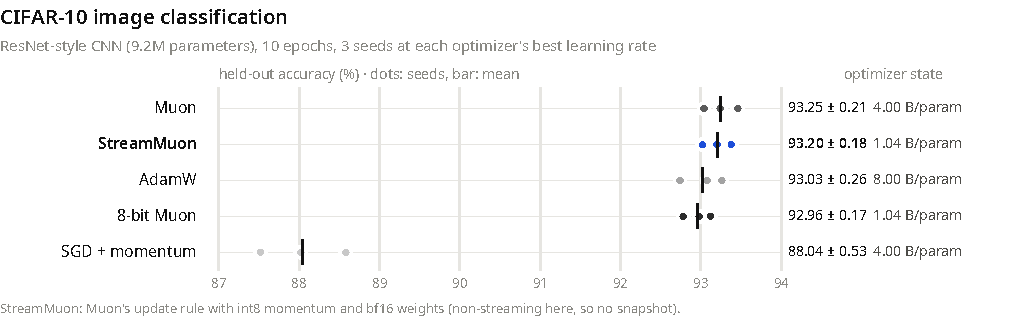
\includegraphics[width=\linewidth]{fig/f5_cifar.pdf}
\caption{CIFAR-10 held-out accuracy: each seed (dots), mean (bar) and mean $\pm$ sample sd, with the optimizer state each
method keeps.}
\label{fig:tasks}
\label{fig:cifar}
\end{figure}

\FloatBarrier
\section{Reproducibility details}
\label{app:repro}
\paragraph{113M Transformer.} $d=576$, 30 layers, 9 attention heads with 3 key-value heads (grouped-query), SwiGLU
hidden size 1536, RMSNorm, rotary positions, QK-norm; 113{,}158{,}293 parameters. Context 512 patches, 8 sequences per
micro-batch, 4 micro-batches per update (16{,}384 patches). Seed 0 for single-seed runs; seeds 0--2 for the repeated
113M runs of Muon and the one-byte accumulator (\S\ref{sec:lm}).
\paragraph{Text data.} A fixed mixture of public web, book, math, code and conversation text, plus a small share of
synthetic tasks; the same mixture and order for every arm. Held-out bits per byte on a fixed held-out set of the same
sources.
\paragraph{MoE Transformers.} The dense recipe with every SwiGLU block replaced by a mixture of SwiGLU experts plus
one always-on shared expert of the same width, softmax router, top-2 with normalized gates, no capacity dropping,
load-balancing loss $E\sum_e f_e\bar p_e$ (weight 0.01); experts run as grouped matmuls. Quality: 16 layers of width
576, 8 experts of width 512, 148.6M total parameters, 8 sequences of 512 per micro-batch. Capacity: 16 layers of width
1024 (16 heads, 4 key-value heads), experts of width 1024, 8 / 16 / 24 / 32 / 48 experts (0.51 / 0.91 / 1.31 / 1.71 /
2.52B total), 4 sequences of 512 per micro-batch. Drift: 4 layers of width 192, 16 experts of width 128.
\paragraph{Hardware and software.} NVIDIA RTX 4060 Laptop GPU (8\,GB, 7.67\,GiB usable, 140\,W maximum power limit),
one job at a time; PyTorch 2.13 (CUDA 13.0), Triton 3.7.1. The settings of \method{} and \lite{} are the defaults
of the released code.

\FloatBarrier
\section{Hyperparameters}
$\beta=0.95$, AdamW $\beta_2=0.95$ for non-matrix parameters, decoupled weight decay 0.05, int8 block 128, five quintic
NS iterations (first three fp8), update multiplier $0.2\sqrt{\max(m,n)}$, $\eta=2\times10^{-3}$, clip norm 1.0, warm-up
409.6k tokens then cosine decay, 16{,}384 tokens per update, context 512, $K=4$ micro-batches at 113M and 8 for the MoE capacity
runs.

\FloatBarrier
\section{Cost projection}
\label{app:cost}
Total cost follows compute and token efficiency, not memory alone. Table~\ref{tab:proj} combines both with
stated assumptions (H100, 40\% utilization, \$2 per GPU-hour, close to the cost of owning the hardware once purchase is
amortized; 60\,GB per GPU for training state under full sharding, with the weight-matrix bytes per parameter; tokens scaled by each optimizer's measured efficiency
and GPU-hours by its measured throughput relative to AdamW). Because the efficiencies come from 113M parameters and a
lightly tuned AdamW, we also give a conservative column at the 1.1$\times$ Muon-type speedup reported at 1.2B
parameters~\citep{wen2026fantastic}.

\begin{table}[!htb]
\centering\small
\caption{Projected minimum H100 count and cost to reach AdamW's 20T-token quality for a 70B model. An extrapolation:
token efficiencies come from 113M parameters against a lightly tuned AdamW; the right column assumes the 1.1$\times$
reported at scale.}
\label{tab:proj}
\begin{tabular}{lrrr}
\toprule
optimizer & min.\ GPUs & cost, measured efficiency & cost, efficiency 1.1$\times$ \\
\midrule
AdamW & 19 & \$11.8M & \$11.8M \\
Muon & 14 & \$4.5M & \$11.5M \\
\method{} & 5 & \$4.7M & \$11.0M \\
\lite{} & 4 & \$5.8M & \$11.2M \\
APOLLO-Mini (assumed AdamW-level) & 3 & \$11.8M & \$11.8M \\
\bottomrule
\end{tabular}
\end{table}

\end{document}
